\subsection{Nested Parallelism}

\begin{flushleft}
    \textcolor{Green3}{\faIcon{question-circle} \textbf{How does OpenMP create multiple threads?}}
\end{flushleft}
OpenMP uses a \textbf{fork-join model} of parallel execution. When a thread encounters a \texttt{parallel} construct, the \textbf{thread creates a team composed of itself and some additional} (possibly zero) \textbf{number of threads}. The encountering \textbf{thread becomes the \emph{master} of the new team}. The \textbf{other threads of the team are called \emph{slave}} threads of the team.

\begin{figure}[!htp]
    \centering
    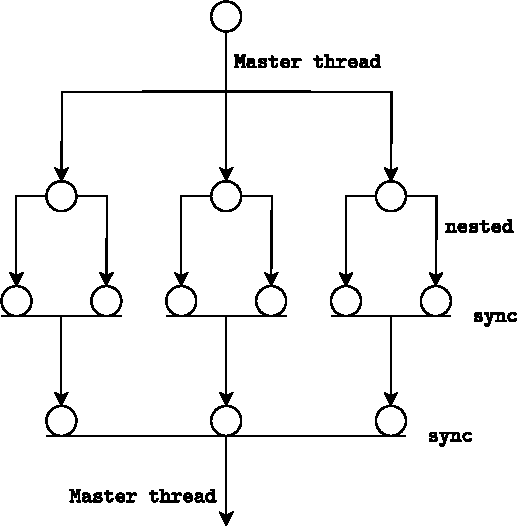
\includegraphics[width=.6\textwidth]{img/openmp-fork-join-1.pdf}
    \caption{OpenMP fork-join model.}
\end{figure}

\begin{flushleft}
    \textcolor{Green3}{\faIcon{question-circle} \textbf{What is the life history of each thread (\emph{slave}) created?}}
\end{flushleft}
All team members execute the code inside the \texttt{parallel} construct. When a thread finishes its work within the parallel construct, it waits at the implicit barrier at the end of the parallel construct. When all team members have arrived at the barrier, the threads can leave the barrier. The \emph{master} thread continues execution of user code beyond the end of the \texttt{parallel} construct, while the \emph{slave} threads wait to be summoned to join other teams.

\highspace
OpenMP \textbf{parallel regions can be nested inside each other}. If nested parallelism is:
\begin{itemize}
    \item \textbf{Disabled}, then the \textbf{new team} created by a thread encountering a parallel construct inside a parallel region \textbf{consists only of the encountering thread}.
    \item \textbf{Enabled}, then the \textbf{new team may consist of more than one thread}.
\end{itemize}

\newpage

\begin{flushleft}
    \textcolor{Green3}{\faIcon{box-open} \textbf{How does OpenMP manage the available threads? Thread Pool}}
\end{flushleft}
The OpenMP runtime library maintains a pool of threads that can be used as \emph{slave} threads in parallel regions. When a thread encounters a parallel construct and needs to create a team of more than one thread, the thread will check the pool and grab idle threads from the pool, making them \emph{slave} threads of the team. The \emph{master} thread might get fewer \emph{slave} threads than it needs if there is not a sufficient number of idle threads in the pool. When the team finishes executing the parallel region, the \emph{slave} threads return to the pool.

\highspace
\begin{flushleft}
    \textcolor{Red2}{\faIcon{bookmark} \textbf{Summary}}
\end{flushleft}
\begin{enumerate}
    \item \textbf{Parallel construct}. Our main thread starts to execute our code. It encounters a \texttt{parallel} construct.
    
    \item \textbf{Pool verification}. The OpenMP library checks its pool of threads. If within its pool of available threads have something of disposable, it allocates the \emph{slave} (thread requested) to the \emph{master} (thread that want to create the team). We refer to a single thread, but obviously this can be extended to multiple thread request (e.g. \emph{master} thread requests 3 threads to OpenMP). Finally, the number of requested \emph{slave}s cannot always be satisfied; OpenMP guarantees the best, so it continues to give the requested threads to the applicants. If it cannot satisfy the request, it returns the maximum number of \emph{slave}s it can satisfy (e.g. \emph{master} requests 4 threads, but OpenMP has a pool of only 2 threads available; therefore it returns 2 \emph{slave}s).
    
    \item \textbf{Assign and start execution}. Ideally, OpenMP returns the number of threads requested by the \emph{master}. Otherwise, it returns the maximum number. The team now consists of the main thread, called the \emph{master}, and its \emph{slave}s. Each member of the team executes the code specified by the programmer within the parallel construct.
    
    \item \textbf{End of execution of a thread}. A thread of the team finishes its work. It can finally rest, and its state changes from "running" to "waiting". It waits for its other thread friends. Each thread has an implicit barrier at the end of the parallel construct.
    
    \item \textbf{Any thread finish}. Finally, each thread finishes its work. The \emph{master} releases each member of the team to the OpenMP library. OpenMP updates its thread pool with the returning threads, and the \emph{master} thread continues its life independently from the released threads.
\end{enumerate}
The previous flow works if and only if nested parallelism is enabled. Otherwise, if a \emph{master} asks to create a new team, it will ignore the request and tell the requester to continue alone.

\newpage

\begin{flushleft}
    \textcolor{Green3}{\faIcon{tools} \textbf{Implementation}}
\end{flushleft}
Nested parallelism can be enabled or disabled by passing true or false as arguments to the runtime function:
\marginpar{
    \href{https://www.openmp.org/spec-html/5.0/openmpsu119.html\#x156-6930003.2.10} {Doc. \faIcon{book}}
}
\begin{openmpbox}[: \texttt{omp\_set\_nested}]
    \begin{lstlisting}[language=C++]
void omp_set_nested(int nested)\end{lstlisting}
\end{openmpbox}

\noindent
We can set a \textbf{default number of threads at different levels of nested parallelism} with:
\begin{center}
    \texttt{OMP\_NUM\_THREADS = [list, of, integers]}
\end{center}
If the nesting level is deeper than the number of entries in the list, the last value is used for all subsequent nested parallel region.

\begin{itemize}
    \item \texttt{OMP\_MAX\_ACTIVATE\_LEVELS} defines the upper \textbf{limit on the number of active parallel regions that may be nested}.

    \item \texttt{OMP\_THREAD\_LIMIT} \textbf{avoids} that recursive applications \textbf{create too many threads}.
\end{itemize}
Finally, since we are in nested parallelism, the thread number returns the thread number partially and not globally, we need other useful functions:
\begin{itemize}
    \item Returns the maximum number of OpenMP threads available in contention group:
    \marginpar{
        \href{https://www.openmp.org/spec-html/5.0/openmpsu123.html\#x160-7180003.2.14} {Doc. \faIcon{book}}
    }
    \begin{openmpbox}[: \texttt{omp\_get\_thread\_limit}]
        \begin{lstlisting}[language=C++]
int omp_get_thread_limit()\end{lstlisting}
    \end{openmpbox}

    \item Returns the maximum number of nested active parallel regions when the innermost parallel region is generated by the current task.
    \marginpar{
        \href{https://www.openmp.org/spec-html/5.0/openmpsu126.html\#x163-7370003.2.17} {Doc. \faIcon{book}}
    }
    \begin{openmpbox}[: \texttt{omp\_get\_max\_active\_levels}]
        \begin{lstlisting}[language=C++]
int omp_get_max_active_levels()\end{lstlisting}
    \end{openmpbox}
    
    \item Limits the number of nested active parallel regions when a new nested parallel region is generated by the current task.
    \marginpar{
        \href{https://www.openmp.org/spec-html/5.0/openmpsu125.html\#x162-7300003.2.16} {Doc. \faIcon{book}}
    }
    \begin{openmpbox}[: \texttt{omp\_set\_max\_active\_levels}]
        \begin{lstlisting}[language=C++]
void omp_set_max_active_levels(int $\emph{max\_levels}$)\end{lstlisting}
    \end{openmpbox}
    
    \newpage

    \item Returns the number of nested parallel regions on the device that enclose tha task containing the call.
    \marginpar{
        \href{https://www.openmp.org/spec-html/5.0/openmpsu127.html\#x164-7430003.2.18} {Doc. \faIcon{book}}
    }
    \begin{openmpbox}[: \texttt{omp\_get\_level}]
        \begin{lstlisting}[language=C++]
int omp_get_level()\end{lstlisting}
    \end{openmpbox}
    
    \item Returns the number of active, nested parallel regions on the device enclosing the task containing the call.
    \marginpar{
        \href{https://www.openmp.org/spec-html/5.0/openmpsu130.html\#x167-7610003.2.21} {Doc. \faIcon{book}}
    }
    \begin{openmpbox}[: \texttt{omp\_get\_active\_level}]
        \begin{lstlisting}[language=C++]
int omp_get_active_level()\end{lstlisting}
    \end{openmpbox}
    
    \item Returns, for given nested level of the current thread, the thread number of the ancestor of the current thread.
    \marginpar{
        \href{https://www.openmp.org/spec-html/5.0/openmpsu128.html\#x165-7490003.2.19} {Doc. \faIcon{book}}
    }
    \begin{openmpbox}[: \texttt{omp\_get\_ancestor\_thread\_num}]
        \begin{lstlisting}[language=C++]
int omp_get_ancestor_thread_num(int $\emph{level}$)\end{lstlisting}
    \end{openmpbox}
    
    \item Returns, for a given nested level of the current thread, the size of the thread team to which the ancestor of the current thread belongs.
    \marginpar{
        \href{https://www.openmp.org/spec-html/5.0/openmpsu129.html\#x166-7550003.2.20} {Doc. \faIcon{book}}
    }
    \begin{openmpbox}[: \texttt{omp\_get\_team\_size}]
        \begin{lstlisting}[language=C++]
int omp_get_team_size(int $\emph{level}$)\end{lstlisting}
    \end{openmpbox}
\end{itemize}